\chapter{Results}

\section{Screenshots of the Application Interface}

\begin {enumerate}
\item First time app Users will be authenticated via PIN received through the message on NGO Registration.
\begin{figure}[here]
\begin{center}   
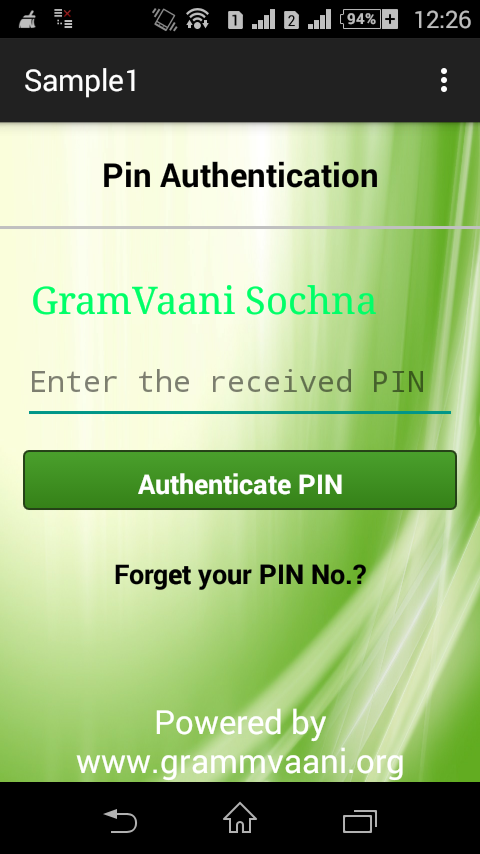
\includegraphics[scale=0.3]{pin_authenticate}
\caption{Pin Authentication}
\label{fig:pin_authenticate}
\end{center}
\end{figure}

\item Online User Registration by the NGO sends a message on registered number for authentication.
\begin{figure}[here]
\begin{center}   
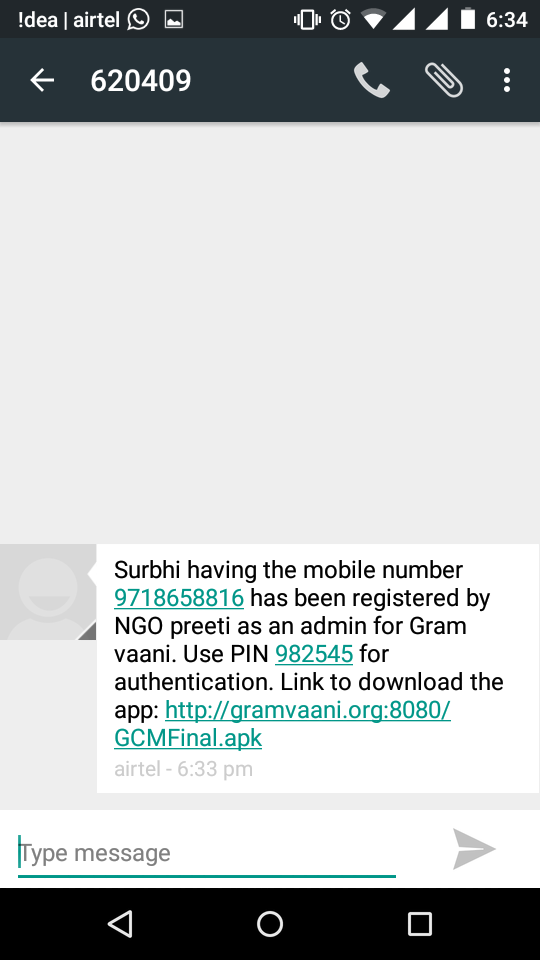
\includegraphics[scale=0.3]{authenticatemsg}
\caption{Message for Pin Authentication}
\label{fig:authenticatemsg}
\end{center}
\end{figure}

\item User can retrieve PIN by clicking on Forget PIN option.
\begin{figure}[here]
\begin{center}   
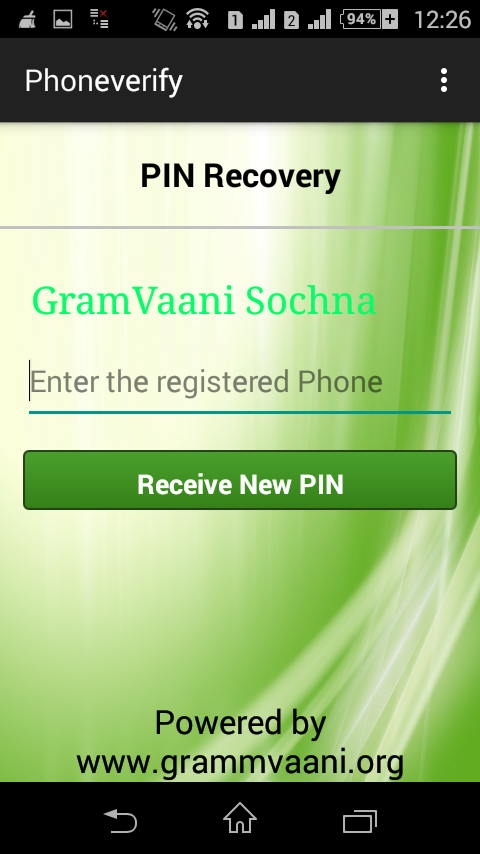
\includegraphics[scale=0.3]{pin_recovery}
\caption{Pin Recovery}
\label{fig:pin_recovery}
\end{center}
\end{figure}

\item User will be provided with the following options.
\begin{figure}[here]
\begin{center}   
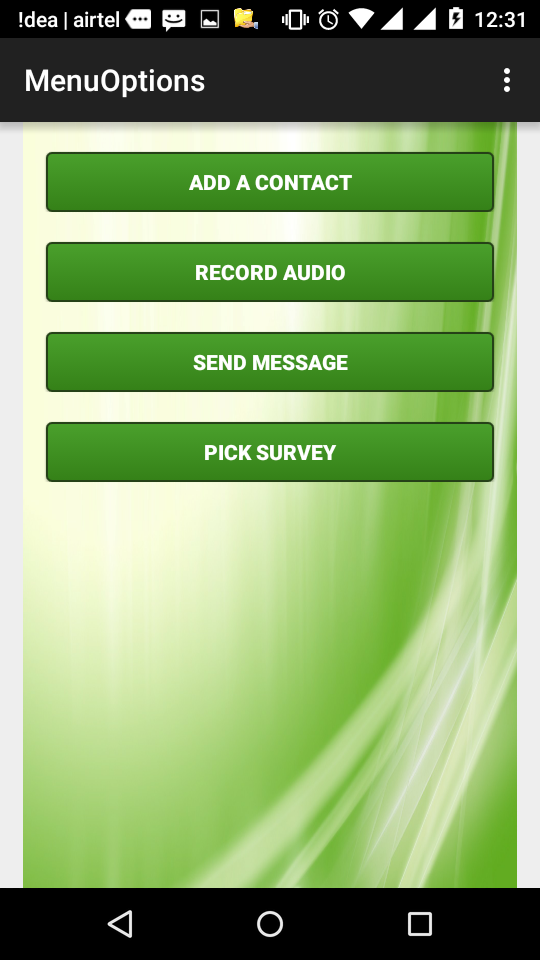
\includegraphics[scale=0.3]{menuoptions}
\caption{Use Cases}
\label{fig:menuoptions}
\end{center}
\end{figure}

\item User can record audio by choosing audio format.
\begin{figure}[here]
\begin{center}   
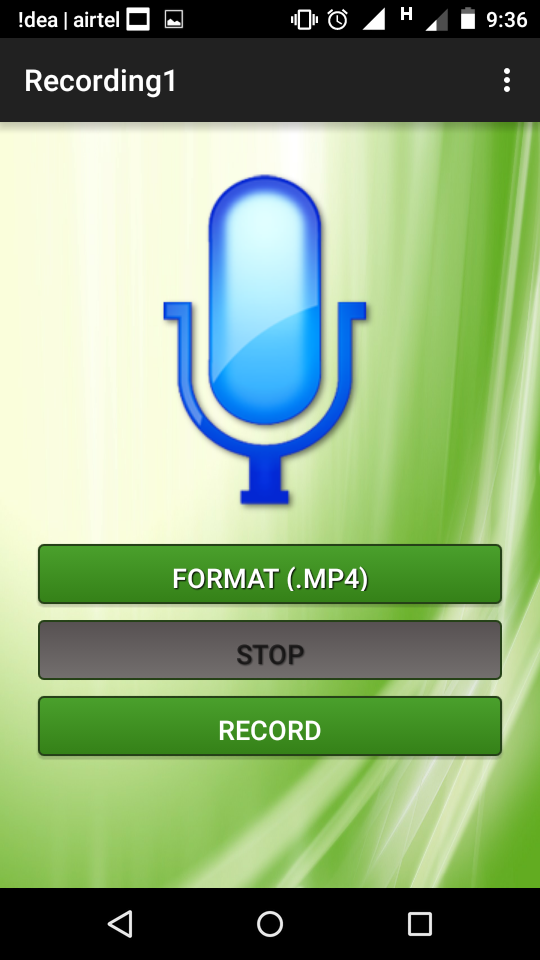
\includegraphics[scale=0.3]{audio1}
\caption{Record Audio}
\label{fig:audio1}
\end{center}
\end{figure}

\item User can choose to either save\/send\/discard an audio message.
\begin{figure}[here]
\begin{center}   
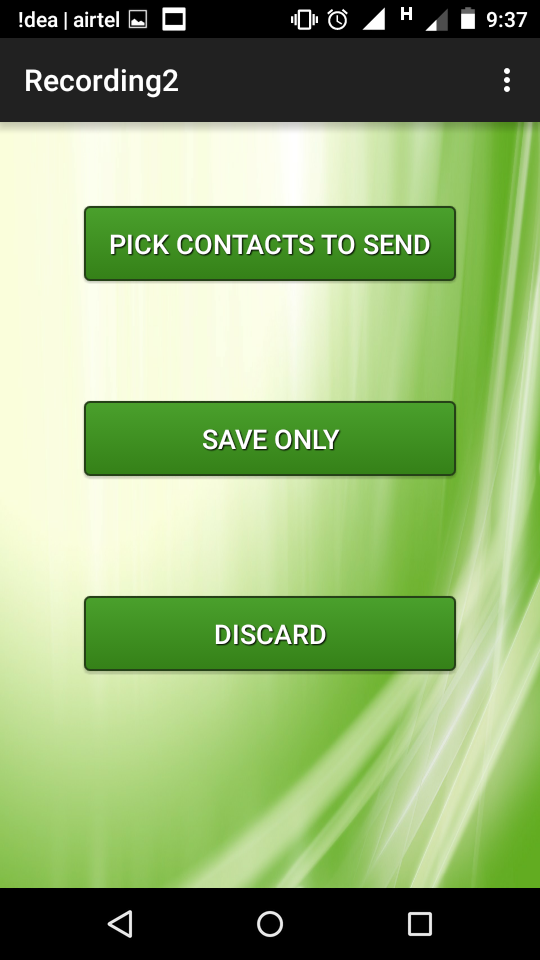
\includegraphics[scale=0.3]{audio2}
\caption{Options After Recording Audio}
\label{fig:audio2}
\end{center}
\end{figure}

\item User can speak a message or type the message to send.
\begin{figure}[here]
\begin{center}   
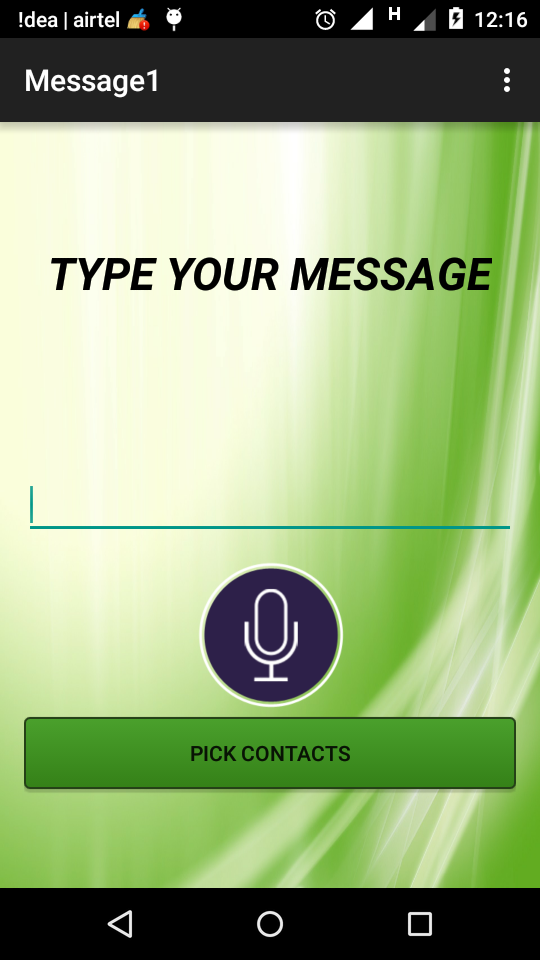
\includegraphics[scale=0.3]{msg1}
\caption{Speak/Type Message}
\label{fig:msg1}
\end{center}
\end{figure}

\item User can view all the active survey names of the GramVaani Server.
\begin{figure}[here]
\begin{center}   
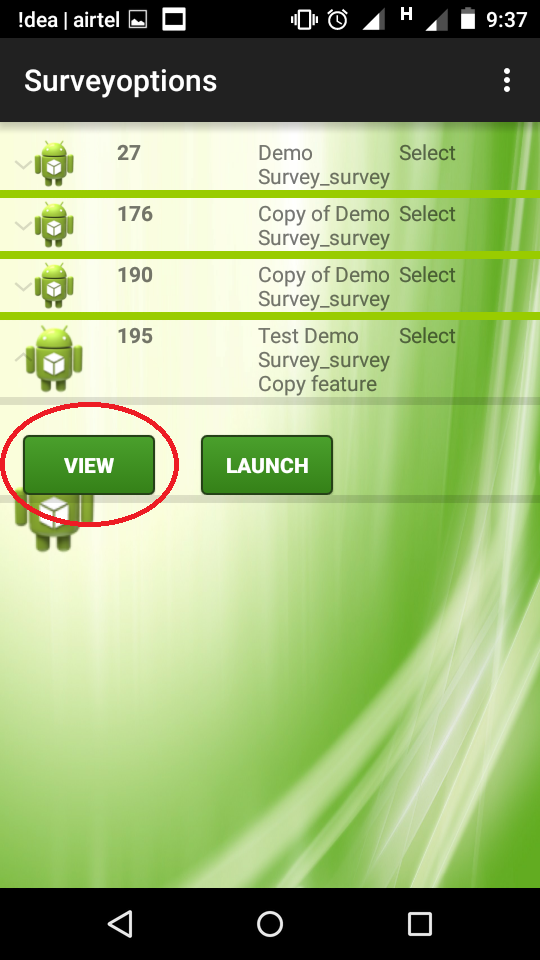
\includegraphics[scale=0.3]{viewlaunchsurvey}
\caption{List of Active Surveys}
\label{fig:viewlaunchsurvey}
\end{center}
\end{figure}

\item User can view a particular survey with all survey questions on selection.
\begin{figure}[here]
\begin{center}   

\includegraphics[scale=0.3]{viewsurvey}
\caption{View a Particular Survey}
\label{fig:viewsurvey}
\end{center}
\end{figure}

\item User can choose the target people among his phone callers, GV callers, Mobile Vaani Recent Callers and GV groups.
\begin{figure}[here]
\begin{center}   
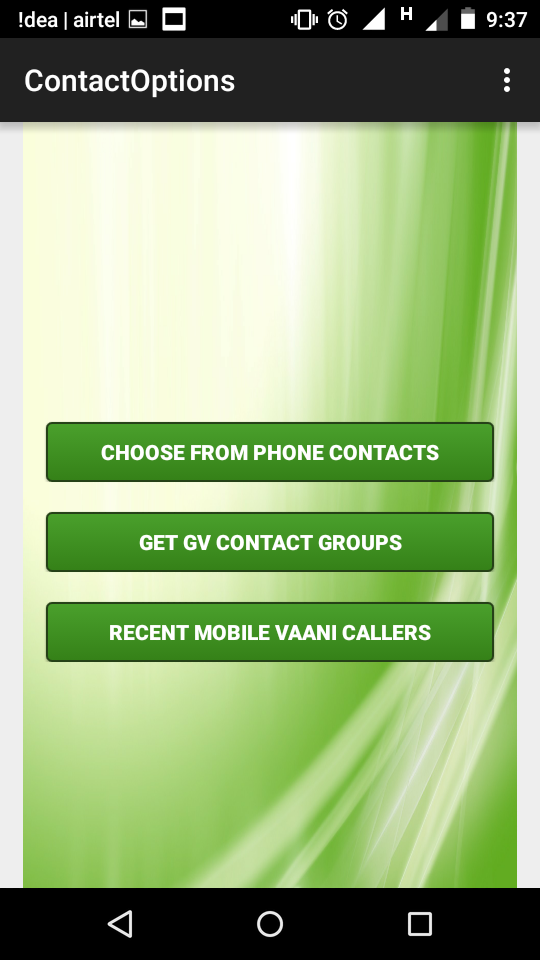
\includegraphics[scale=0.3]{contactoptions}
\caption{Choose Target Contacts}
\label{fig:contactoptions}
\end{center}
\end{figure}

\item Multiple GV contact groups can be choosen as the target people.
\begin{figure}[here]
\begin{center}   
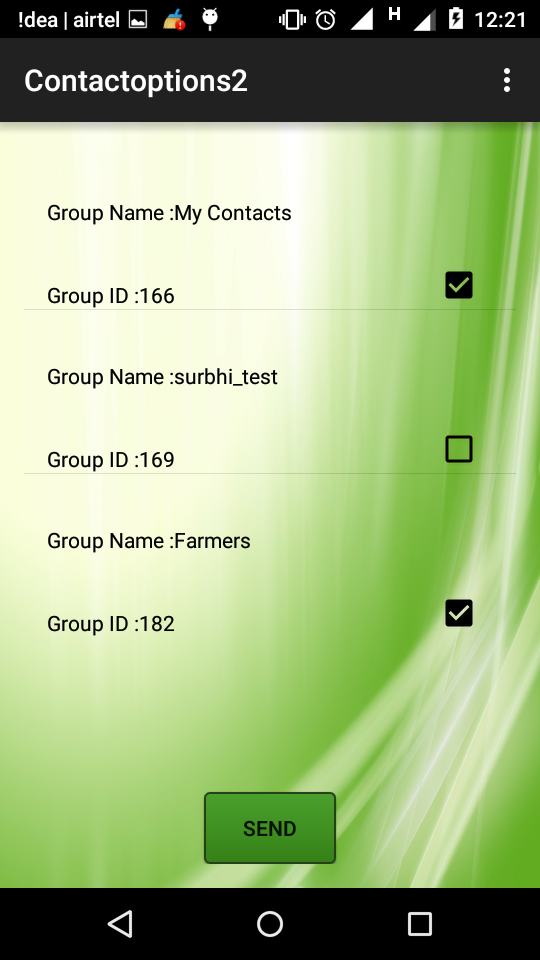
\includegraphics[scale=0.3]{contactgroups}
\caption{GV Contact Groups}
\label{fig:contactgroups}
\end{center}
\end{figure}

\item Multiple phone contacts can be choosen as the target people.
\begin{figure}[here]
\begin{center}   
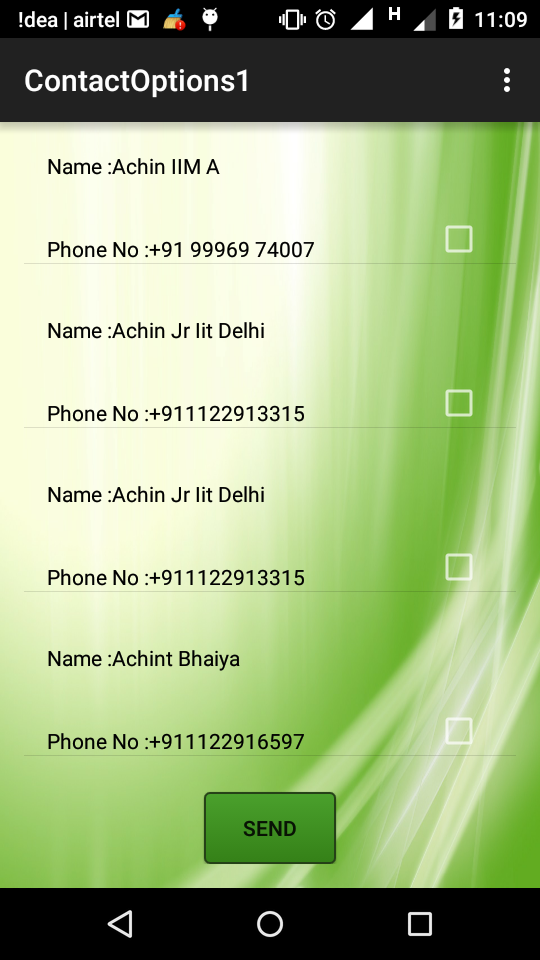
\includegraphics[scale=0.35]{phonecontacts}
\caption{Phone Contacts}
\label{fig:phonecontacts}
\end{center}
\end{figure}

\end{enumerate}

\section{Screenshot of the GramVaani Web Instance}

\begin{enumerate}

\item GramVaani Graphical Web Portal Instance
\begin{figure}[here]
\begin{center}   
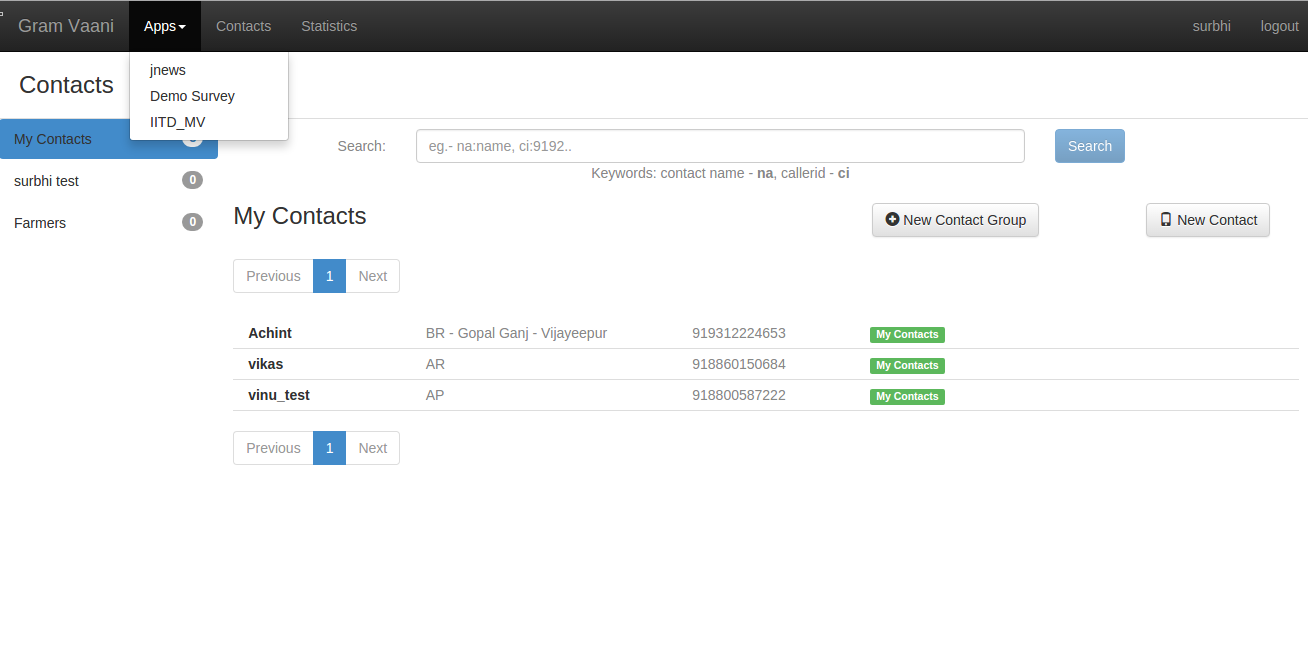
\includegraphics[scale=0.3]{gvinstance1}
\caption{GramVaani Web Instance}
\label{fig:gvinstance1}
\end{center}
\end{figure}


\end{enumerate}




\section{Screenshots of the Web Portal}

\begin{enumerate}
\item Home Page of the Web Portal for NGO's Registration and other functionalities
\begin{figure}[here]
\begin{center}   
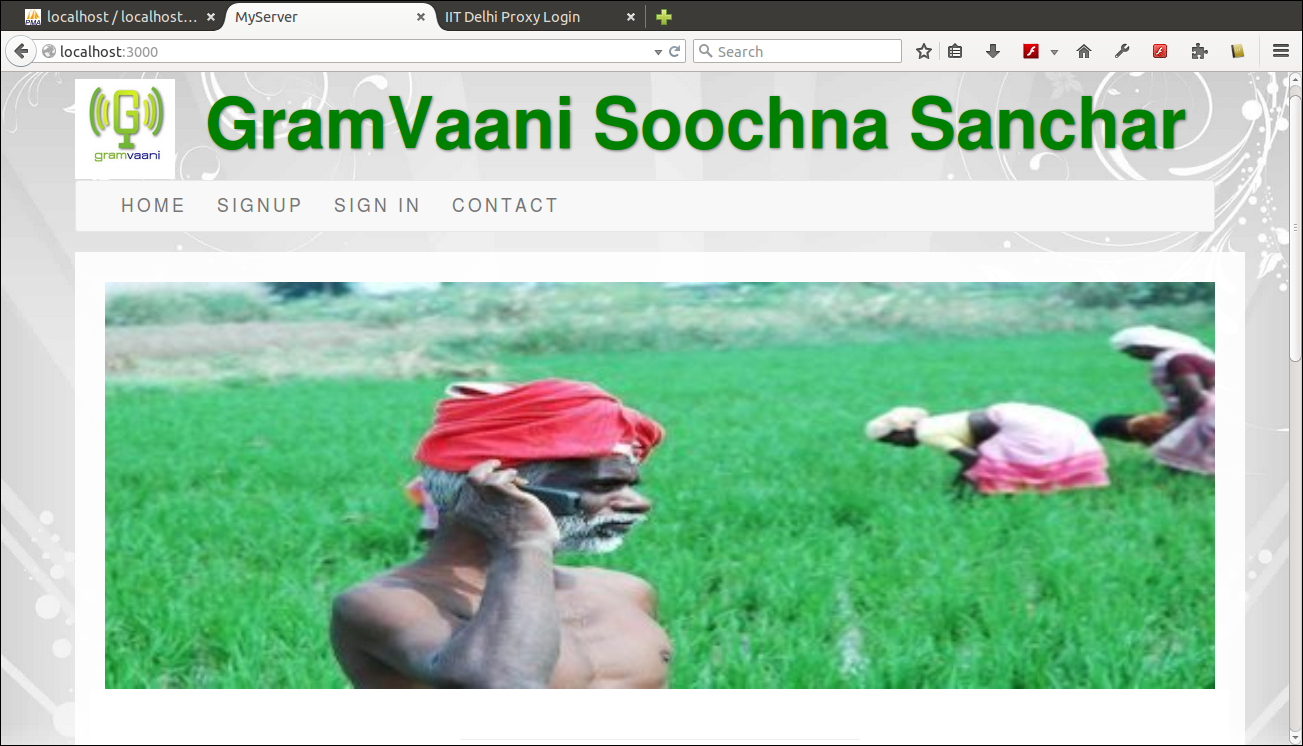
\includegraphics[scale=0.3]{w1}
\caption{GramVaani Soochna Sanchar Home Page}
\label{fig:w1}
\end{center}
\end{figure}


\item NGO's Login Page
\begin{figure}[here]
\begin{center}   
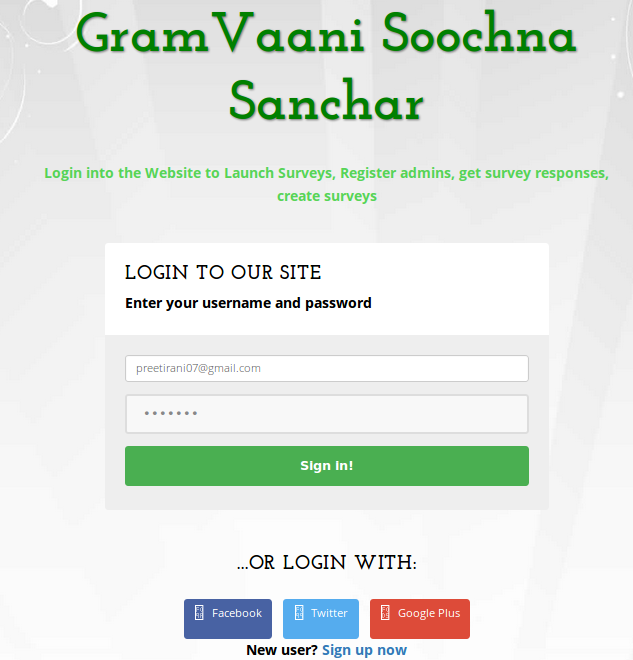
\includegraphics[scale=0.3]{w10}
\caption{NGO's Login Page}
\label{fig:w10}
\end{center}
\end{figure}



\item Use cases provided to the NGO users
\begin{figure}[here]
\begin{center}   
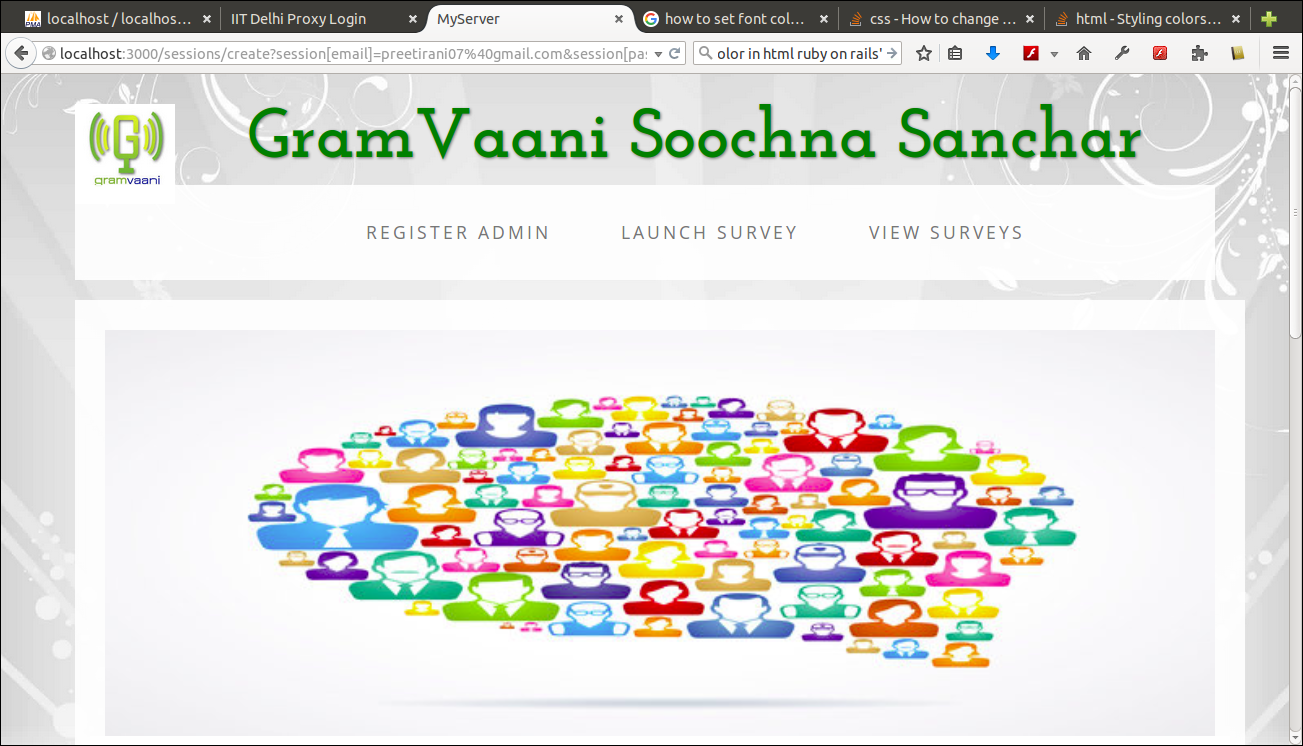
\includegraphics[scale=0.3]{w14}
\caption{Use Cases of NGO Personnel}
\label{fig:w14}
\end{center}
\end{figure}



\item Web Online form for Admins Registration and Authentication
\begin{figure}[here]
\begin{center}   
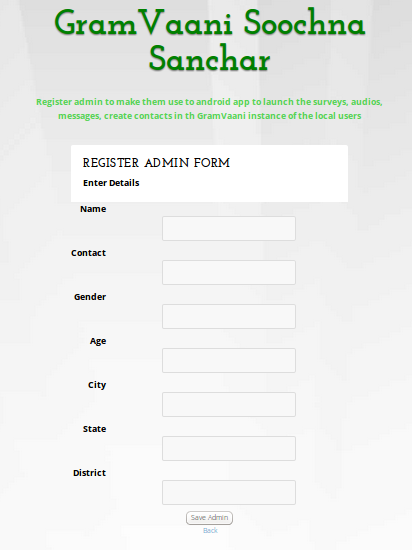
\includegraphics[scale=0.3]{w15}
\caption{Admin's Registration Form}
\label{fig:w15}
\end{center}
\end{figure}




\item NGO Personnel can launch a particular survey for a particular district.
\begin{figure}[here]
\begin{center}   
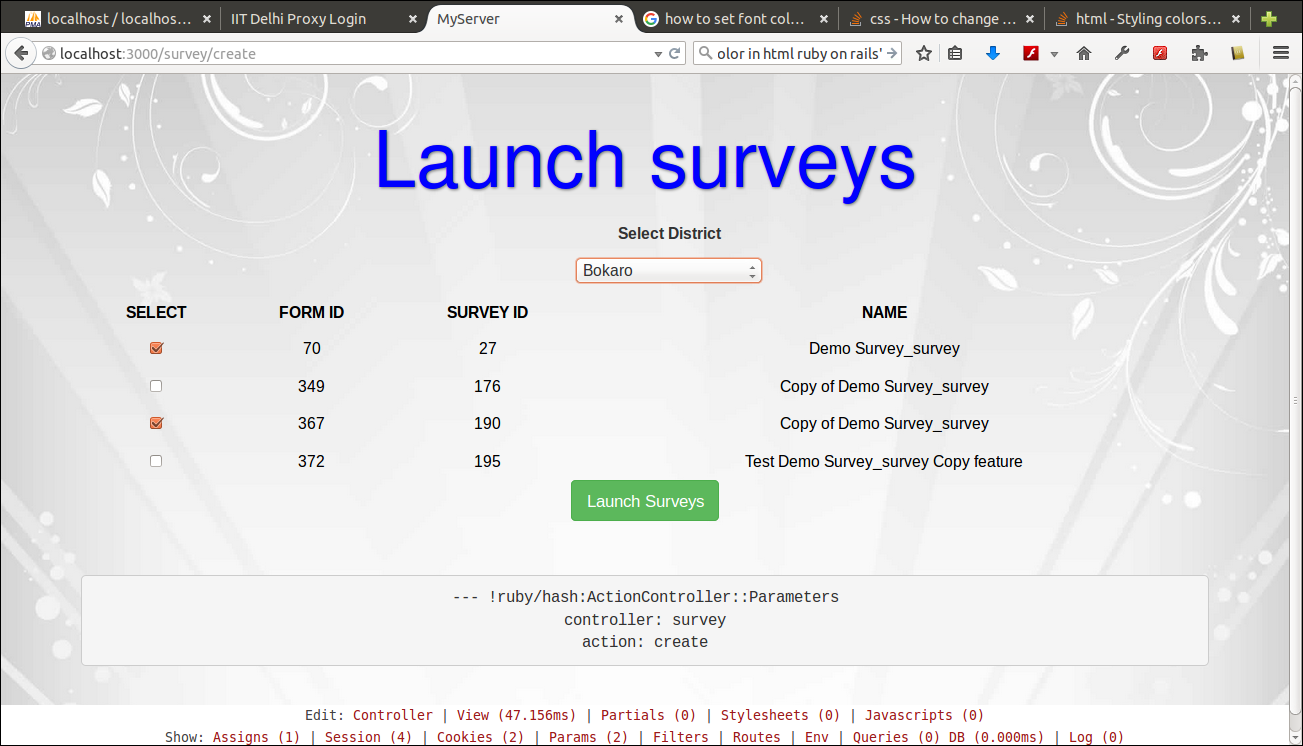
\includegraphics[scale=0.3]{w16}
\caption{Launch Survey in a District}
\label{fig:w16}
\end{center}
\end{figure}


\item NGO Personnel can view all the active surveys along with viewing current responses and survey questions.
\begin{figure}[here]
\begin{center}   
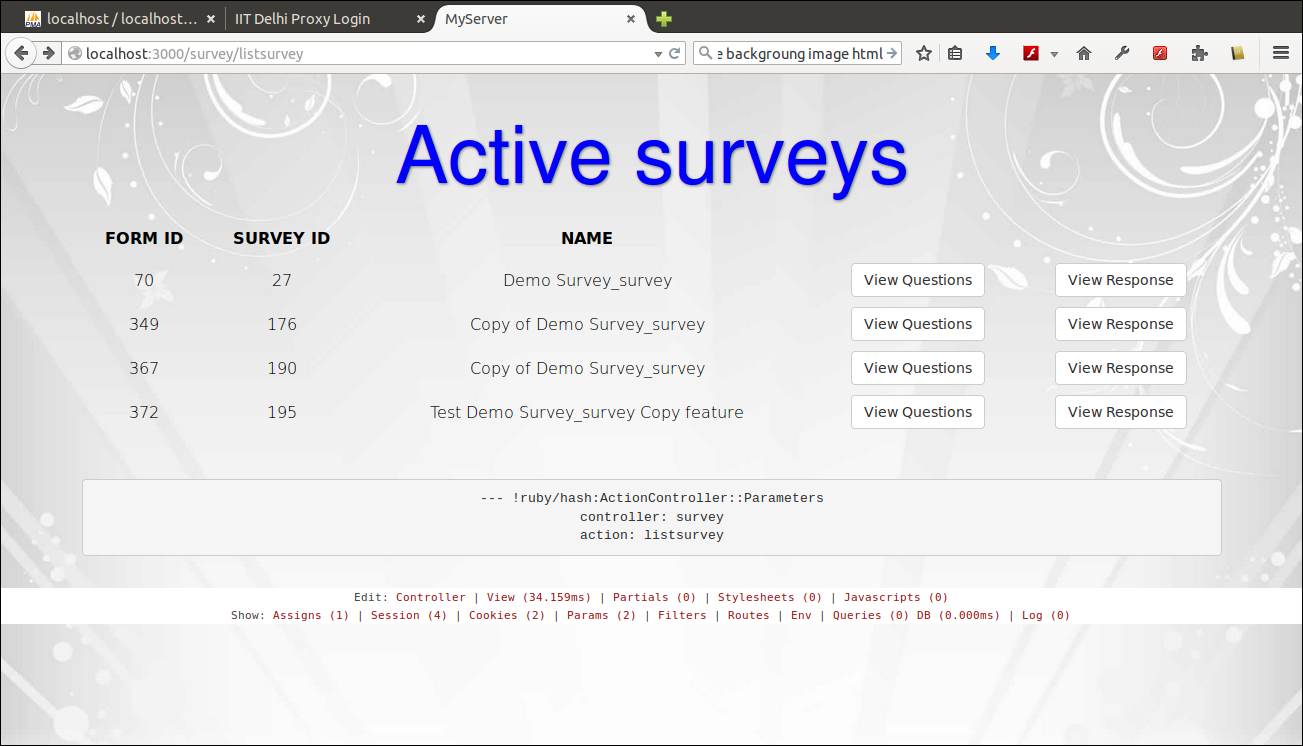
\includegraphics[scale=0.3]{w13}
\caption{View Active Surveys}
\label{fig:w13}
\end{center}
\end{figure}


\item NGO Personnel can view the responses of the active survey.
\begin{figure}[here]
\begin{center}   
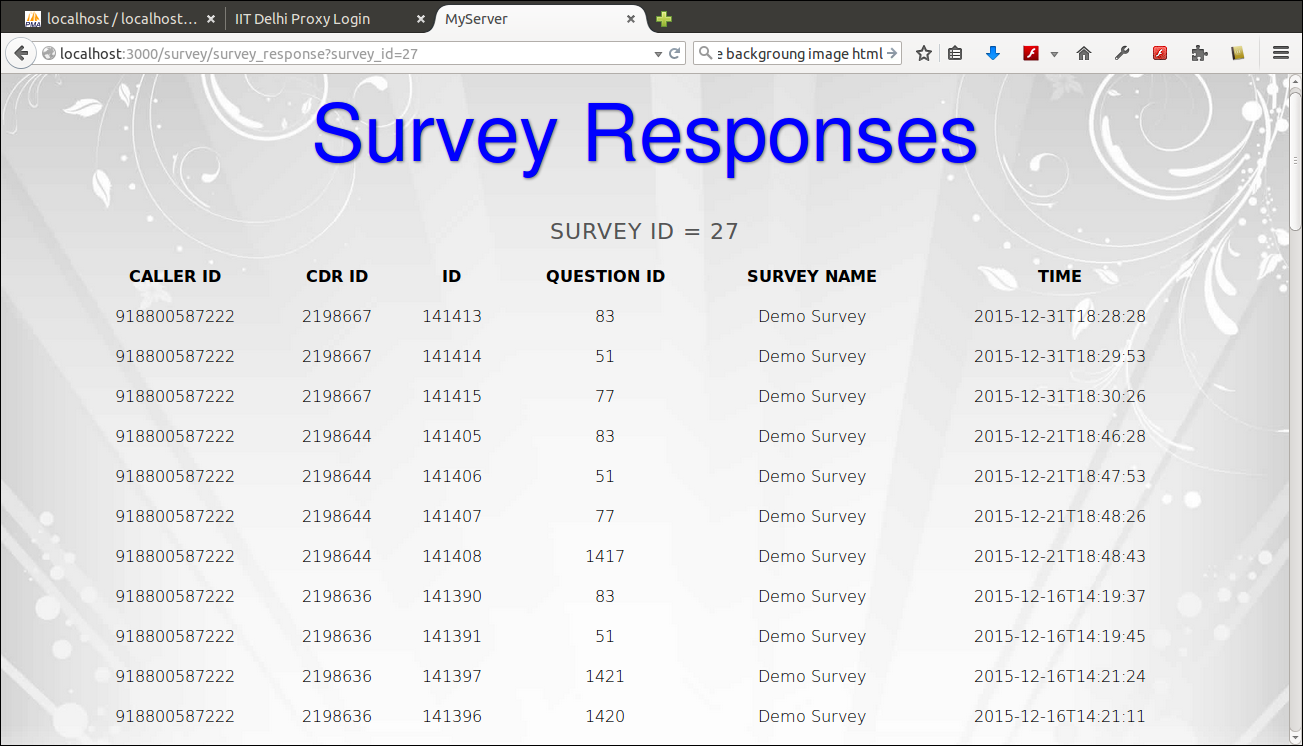
\includegraphics[scale=0.3]{w11}
\caption{View Active Survey Responses}
\label{fig:w11}
\end{center}
\end{figure}


\item NGO Personnel can view the text questions of the active survey.
\begin{figure}[here]
\begin{center}   
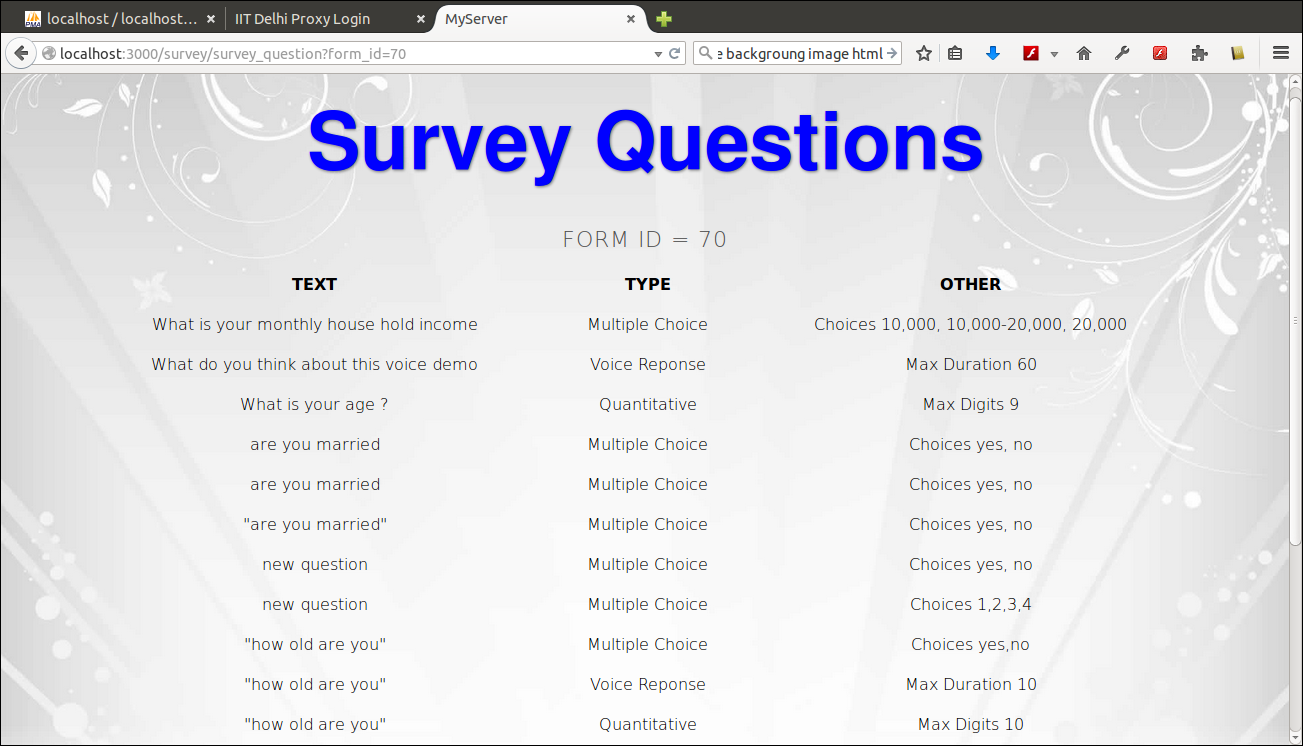
\includegraphics[scale=0.3]{w12}
\caption{View Active Survey Questions}
\label{fig:w12}
\end{center}
\end{figure}
 
\end{enumerate}













